\section{Mechanics}
\showtoc

\subsection{Hybrid Systems}
\begin{frame}[t]
  \frametitle{Bipedal Models}
  \begin{figure}
    \centering
    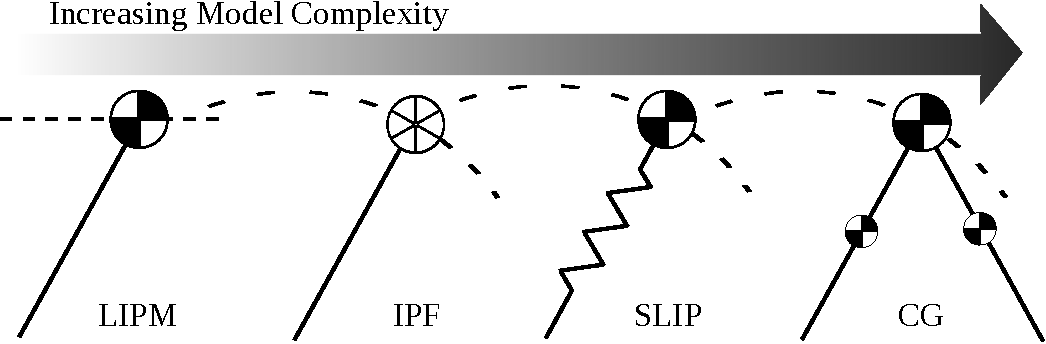
\includegraphics[width=.9\textwidth]{biped-models}
  \end{figure}
  \begin{itemize}
  \item Bipedal locomotion has been studied with a variety of models.
  \item Pendulum models consider massless legs with no impacts.
  \item Kinematic chains are markedly more complex than pendula.
  \end{itemize}
\end{frame}

\begin{frame}[t]
  \frametitle{Modeling Hybrid Systems}
  \begin{columns}
    \begin{column}{.63\textwidth}
      \begin{definition}
        A \alert{hybrid control system} is a tuple \vspace{-.3cm}
        $$\HCS = \hcsystem, \vspace{-.4cm}$$
        where
        \begin{itemize}
        \item
          $\Domain \subset \X$ is the \blue{domain of admissibility} with state space $\X$,
        \item
          $\ControlSet$ is a set of \blue{admissible controls},
        \item
          $\Guard$ is a \blue{guard} or \blue{switching surface},
        \item
          $\ResetMap$ is a smooth \blue{reset map},
        \item
          $(\xf, \xg)$ is a \blue{control system} on $\Domain$: \vspace{-3mm}
          \begin{align*}
            \dx = \xf(\x) + \xg(\x) \, \uu.
          \end{align*}
        \end{itemize}
      \end{definition}
    \end{column}
    \begin{column}{.4\textwidth}
      \begin{figure}    
        \centering
        \def\svgwidth{.8\columnwidth}
        \input{../figs/simple_hybrid_system.eps_latex}
      \end{figure}
      \vspace{-1em}
      A \alert{simple hybrid system}:\vspace{-.5em}
      $$\HS = \hsystem$$
    \end{column}
  \end{columns}
\end{frame}

\begin{frame}[t]
  \frametitle{Lagrangian Systems}
  Mechanical systems are defined by:
  \begin{itemize}
  \item Kinetic energy, $T : T\sQ \to \Rnn$,\\
  \item Potential energy, $U : \sQ \to \R$,
  \end{itemize}
  which together comprise the Lagrangian,
  \begin{align*}
    \Lagrangian\argsqdq = T\argsqdq - U\argsqdq.
  \end{align*}
  Dynamical motion in such a system with external forcing $\mathcal{F} = B\argsq u$ is governed by the Euler--Lagrange equation:
  \begin{align*}
    \frac{d}{dt} \pd{\Lagrangian}{\dq} - \pd{\Lagrangian}{\q} = B\argsq u.
  \end{align*}
\end{frame}

\begin{frame}[t]

  \frametitle{Swing Phase Dynamics}
  \begin{columns}
    \begin{column}{.55\textwidth}
      For Lagrangian $\Lagrangian$ with coordinates
      \begin{align*}
        \x = \argsqdq \in T\ConfigurationSpace,
      \end{align*}
      the dynamic model has the form
      \begin{align*}
        \M\argsq \, \ddq + \C\argsqdq \, \dq + \G\argsq = \B\argsq \, \uu,
      \end{align*}
      or $\dx = \xf\argsqdq+ \xg\argsq \, \uu,$ with
      \begin{align*}
        \xf\argsqdq &= \left(\!\!\begin{array}{c}
            \dq\\
            \M^{-1}\argsq (-\C\argsqdq \, \dq - \G\argsq)
          \end{array}\!\!\right),\\
        \xg(\q) &= \left(\!\!\begin{array}{c}
            \mathbf{0}_{m \times m}\\
            \M^{-1}(\q) \B(\q)
          \end{array}\!\!\right).
      \end{align*}
    \end{column}\!\!
    \begin{column}{.45\textwidth}
      \begin{figure}
        \centering
        \vspace{-10mm}
        \caption{Physical configuration}
        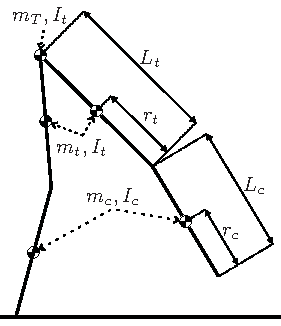
\includegraphics[width = 1.0\columnwidth]{pointfoot_robot_config}
      \end{figure}
    \end{column}
  \end{columns}
\end{frame}

\begin{frame}[t]
  \frametitle{Impact Dynamics}
  Introduce extended coordinates $\qe = (X, \q) \in \mathrm{SE}(3) \times \ConfigurationSpace$ which contains the kinematics of a reference point on the robot. Angular momentum balance based on H{\"u}rm{\"u}zl{\"u} and Marghitu:
  \begin{massump}
    \begin{itemize}
    \item Rigid-body plastic impacts
    \item Enough friction to prevent slipping
    \item Motors do not produce impulses
    \item No instantaneous change in configuration, i.e., $\qe^{-} = \qe^{+}$
    \end{itemize}
  \end{massump}
  Under these assumptions, the discrete dynamics satisfies
  \begin{align*}
    \left[\begin{array}{c c}
        \D_{e}(\qe) & -\Jacobian^{T}(\qe)\\
        \Jacobian(\qe) & \mathbf{0}_{3 \times 3}
      \end{array}\right]
    \left[\begin{array}{c}
        \dq^{+}\\
        \delta F(\qe, \dqe)
      \end{array}\right]
    = \left[\begin{array}{c c}
        \D_{e}(\qe) \, \dqe^{-}\\
        \mathbf{0}_{3}
      \end{array}\right].
  \end{align*}
\end{frame}

\subsection{Solutions to Hybrid Systems}
\begin{frame}[t]
  \frametitle{Hybrid Flows}
  A \alert{hybrid flow} of $\HS$ is a tuple
  \begin{align*}
    \chi^{\HS} = \left( \Delta, \mathscr{I}, \mathscr{C} \right),
  \end{align*}
  \vspace{-2em}
  \begin{itemize}
  \item $\Delta = \{0, 1, 2, \ldots\} \subseteq \Nat$ is a finite or infinite \blue{indexing set},
  \item $\mathscr{I} = \{I_{i} \}_{i \in \Delta}$ is a \blue{hybrid interval} where $I_{i} = [\tau_{i}, \tau_{i + 1}]$,
  \item $\mathscr{C} = \{c_{i} \}_{i \in \Delta}$ is a \blue{collection of solutions} of $\xf$, i.e., ${\dot c}_{i}(t) = \xf(c_{i}(t))$ $\forall i \in \Delta$.
  \end{itemize}

  \only<1>{
    \vspace{-1em}
    \begin{figure}
      \centering
      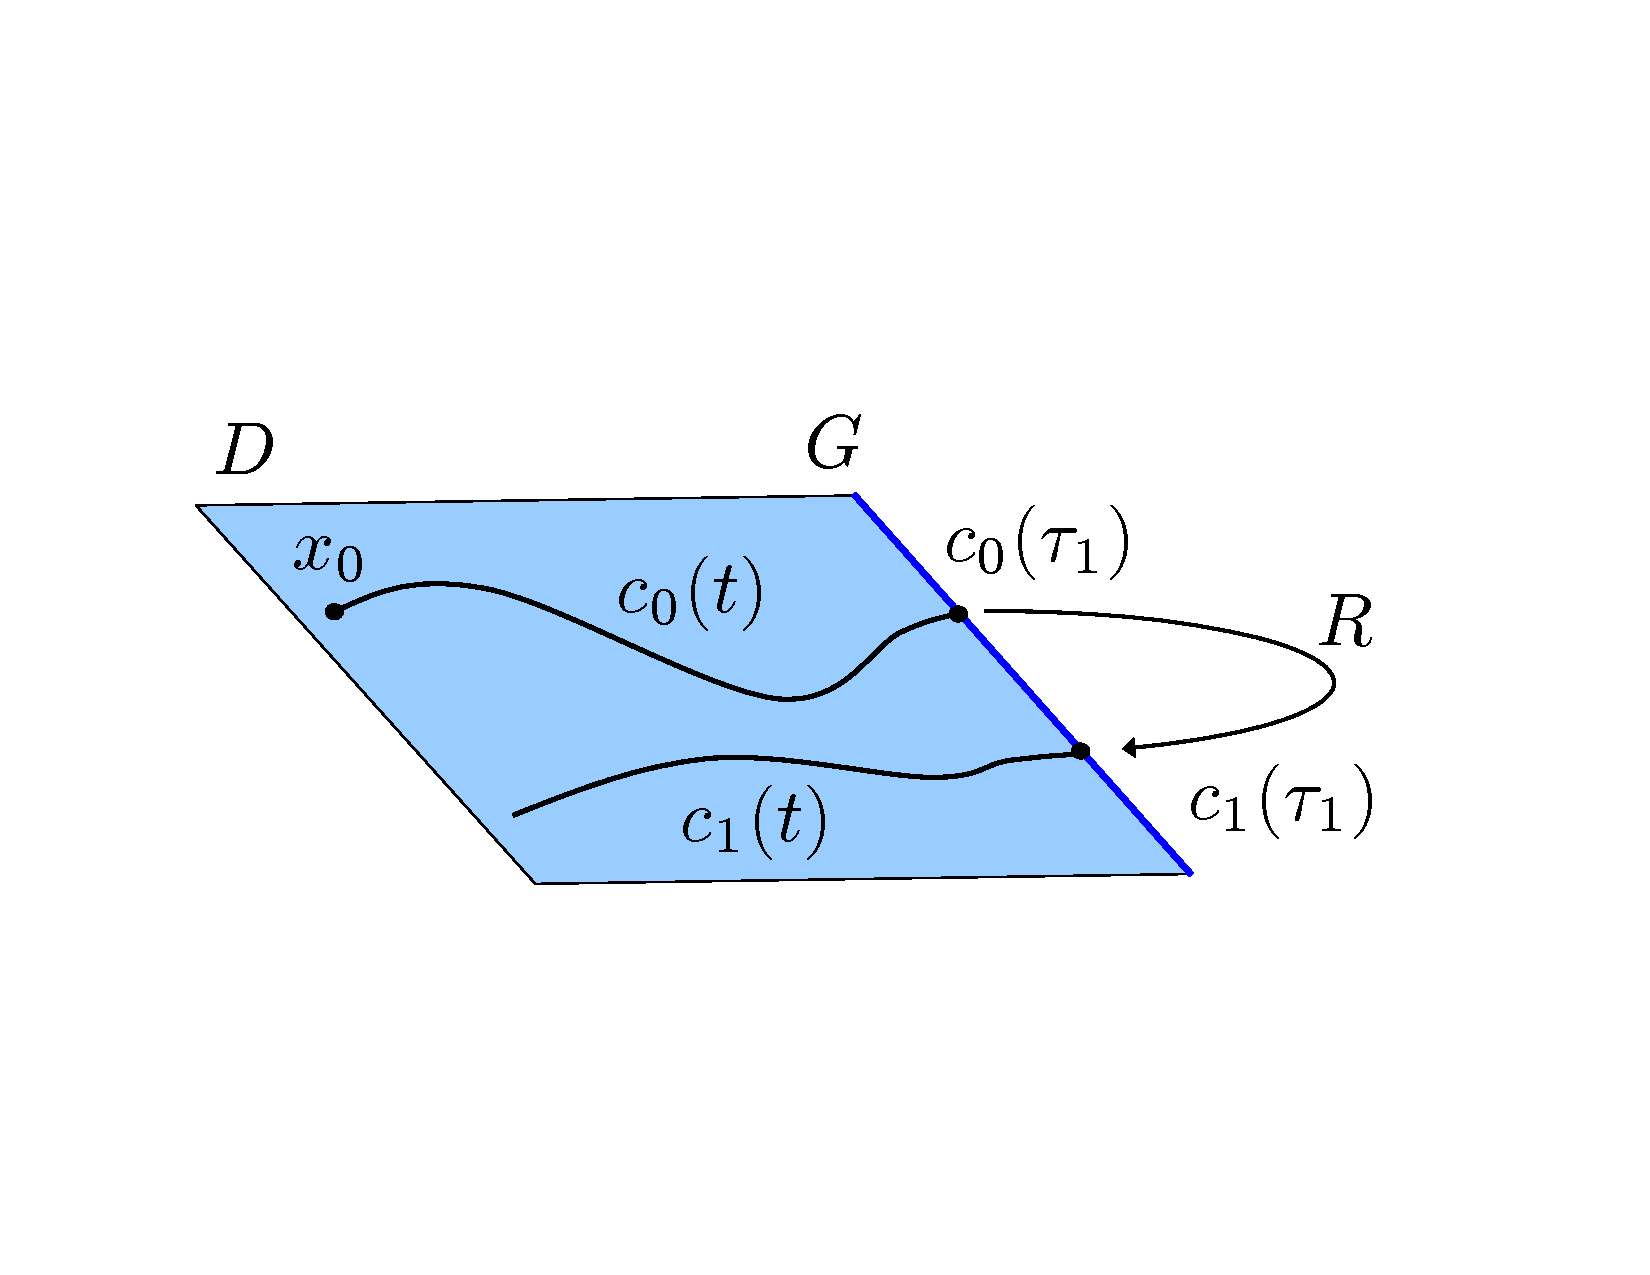
\includegraphics[width=0.5\columnwidth]{hybridflow}
    \end{figure}
    \vspace{-1em}
  }

  \only<2>{
    In addition, for every $i, i + 1 \in \Delta$, it is required that
    \begin{enumerate}
    \item $c_{i}(\tau_{i+1}) \in G$ and
    \item $\Delta(c_{i}(\tau_{i+1})) = c_{i+1}(\tau_{i+1})$
    \end{enumerate}
  }
\end{frame}


\begin{frame}[t]
  \frametitle{Periodic Orbits}
  \begin{figure}    
    \centering
    \def\svgwidth{.45\columnwidth}
    \input{../figs/hybrid_periodic_orbit.eps_latex}
    \caption{A hybrid periodic orbit. Stability is ascertained using the method of Poincar\'e.}
  \end{figure}
\end{frame}

\begin{frame}[t]
  \frametitle{Conservative Systems}
  For a conservative system, total energy is conserved; i.e.:
  \begin{align*}
    \Ec &= T\argsqdq + U\argsq\\
    &= \E(q(0), \dot q(0)) = \E_{0}
  \end{align*}
  Dynamical motion for such a system relies on the interplay between kinetic and potential energy, which is expressed in the Euler-Lagrange equation,
  \begin{align*}
    \frac{d}{dt} \pd{\Lagrangian}{\dq} - \pd{\Lagrangian}{\q} = 0.
  \end{align*}
\end{frame}


\begin{frame}[t]
  \frametitle{The Simplest Example: Passive Compass-Gait Biped}
  \only<1>{
    \begin{columns}
      \column{1.5in}
      Dynamic Model:
      \begin{align*}
        \M\argsq \ddot q + \CG\argsqdq = 0
      \end{align*}
      Control Law:
      \begin{align*}
        \uu = 0.
      \end{align*}
      \column{1.5in}
      \begin{figure}%width=1.0\columnwidth,
        
        \centering
        \def\svgwidth{1.0\columnwidth}
        \input{../figs/cg2d-slope-model.eps_latex}
        \vspace{-2em}
        \caption{Compass-gait biped falling down a slope.}
      \end{figure}
    \end{columns}
  }

  \only<2>{
    \begin{figure}
      \includemedia[
      % width=1.0\columnwidth,
      % height=0.5625\columnwidth,
      %width=1.0\columnwidth,
      %height=0.5\columnwidth,
      width=.9\columnwidth,
      height=0.45\columnwidth,
      addresource=cg2d_slope.mp4,
      activate=pageopen,
      flashvars={source=cg2d_slope.mp4&loop=true&autoPlay=true}
      ]{}{VPlayer9.swf}
      \caption{Stable passive gaits can be found for a range of slopes.}
    \end{figure}    
  }

  \only<3>{
    \begin{figure}
      \centering
      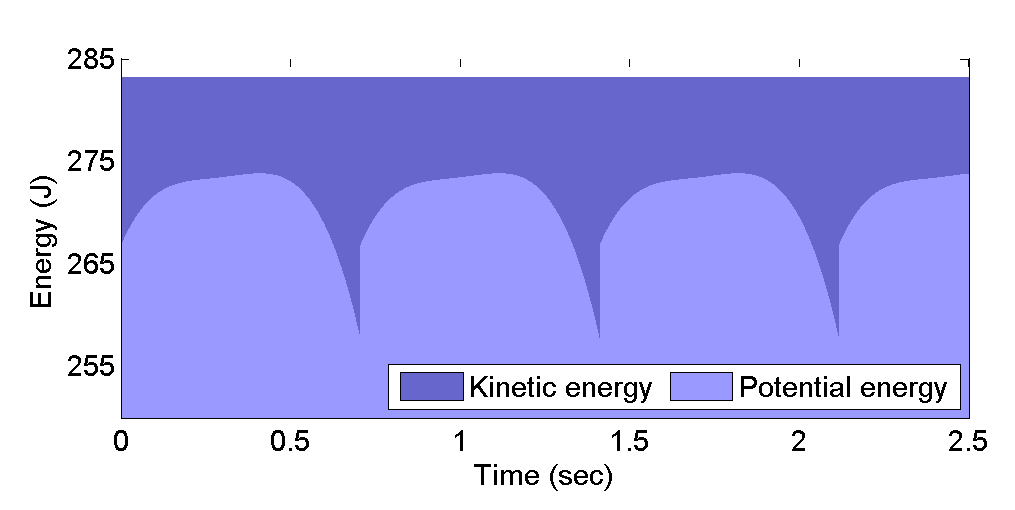
\includegraphics[width=1.0\columnwidth]{energy_cg2d_slope_model}
      \caption{Energy is exchanged between kinetic and potential in form.}
    \end{figure}    
  }
\end{frame}


\begin{frame}[t]
  \frametitle{Nonconservative Systems}
  For a nonconservative system, energy flows out of the system at a rate of $F_{\nc} \cdot dq$. Thus, the following quantity is conserved:
  \begin{align*}
    \Ec &= T\argsqdq + U\argsq - \int_{t_{0}}^{t} \! F_{\nc} \cdot \frac{dq}{d\tau} \ d\tau\\
    &= \E(q(0), \dot q(0)) = \E_{0}
  \end{align*}
  This equation expresses the interplay between kinetic and potential energy and the flow of energy into and out of the system.
\end{frame}


\begin{frame}[t]
  \frametitle{Example: Active Compass-Gait Biped}
  \only<1>{
    \begin{columns}
      \column{1.5in}
      Dynamic Model:
      \begin{align*}
        \M\argsq \ddq + \CG\argsqdq = \B\argsq \uu.
      \end{align*}
      Controlled Symmetries:
      \begin{align*}
        \uu &= \G\argsq - G(\Psi_{\gamma}\argsq)
      \end{align*}
      where $\Psi : \S \times \R \to \sQ$ rotates the frame of gravity by $\gamma$.

      \column{1.5in}
      \begin{figure}
        \centering
        \def\svgwidth{1.0\columnwidth}
        \input{../figs/cg2d-2link-model.eps_latex}
        \vspace{-2em}
        \caption{Compass-gait biped with Controlled Symmetries.}
      \end{figure}
    \end{columns}
  }
  \only<2>{
    \begin{figure}
      \includemedia[
      % width=1.0\columnwidth,
      % height=0.5625\columnwidth,
      width=.9\columnwidth,
      height=0.45\columnwidth,
      addresource=cg2d_2link_simulation.mp4,
      activate=pageopen,
      flashvars={source=cg2d_2link_simulation.mp4&loop=true&autoPlay=true}
      ]{}{VPlayer9.swf}
      \caption{Passive downhill gaits can be translated to flat ground with Controlled Symmetries.}
    \end{figure}    
  }
  \only<3>{
    \begin{figure}
      \centering
      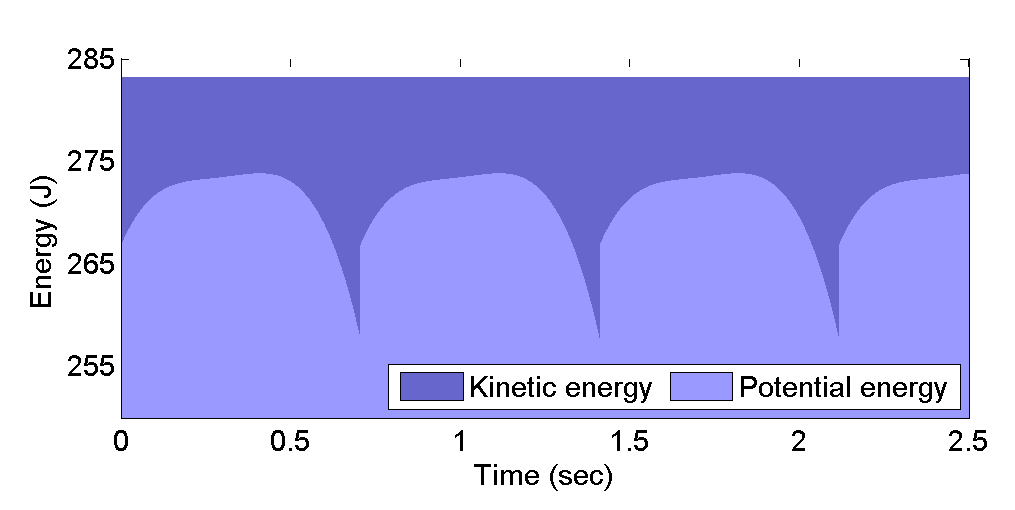
\includegraphics[width=1.0\columnwidth]{energy_cg2d_slope_model}
      \caption{Energy of the shaped system is conserved.}
    \end{figure}    
  }
\end{frame}

\begin{frame}[t]
  \frametitle{Example: 3-Link Biped}
  \only<1>{
    \begin{columns}
      \column{1.5in}
      Dynamic Model:
      \begin{align*}
        \M\argsq \ddq + \CG\argsqdq = \B\argsq \uu
      \end{align*}
      Control Law:
      \begin{align*}
        \uu &= \G\argsq - \G(\Psi\argsq)\\
        \uu_3 &=-k_{d} (\dot \vartheta_{T}^{a})\\
        &\hspace{1.8em} -k_{p} (\vartheta_{T}^{a} - \vartheta_{T}^{d})
      \end{align*}
      \column{1.5in}
      \begin{figure}
        \centering
        \def\svgwidth{1.0\columnwidth}
        \input{../figs/cg2d-3link-model.eps_latex}
        \vspace{-2em}
        \caption{3-link biped configuration.}
      \end{figure}
    \end{columns}
  }

  \only<2>{
    \begin{figure}
      \centering
      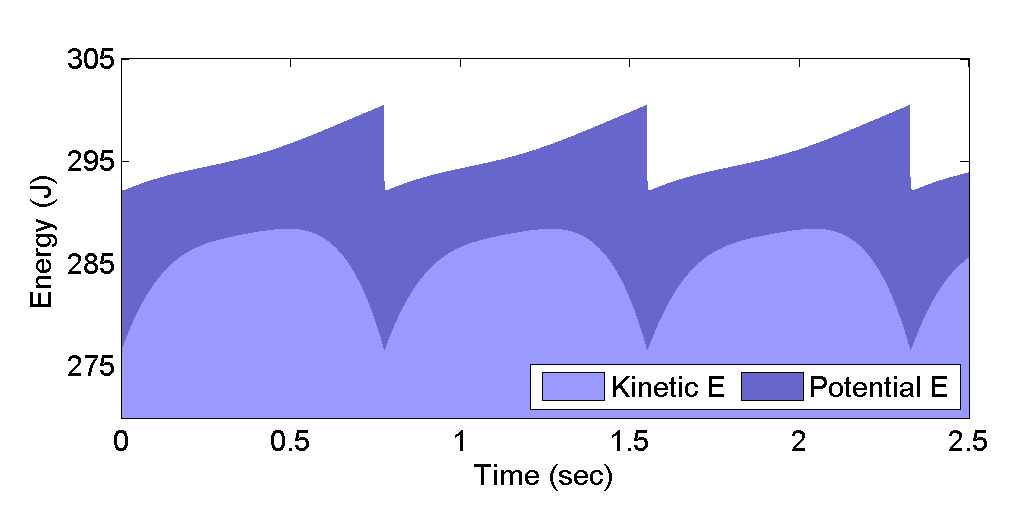
\includegraphics[width=1.0\columnwidth]{energy_cg2d_3link}
      \caption{Energy is not conserved as the controller injects energy.}
    \end{figure}
  }

  \only<3>{
    \begin{figure}
      \includemedia[
      %width=1.0\columnwidth,
      %height=0.5\columnwidth,
      width=.9\columnwidth,
      height=0.45\columnwidth,
      addresource=cg2d_3link_simulation.mp4,
      activate=pageopen,
      flashvars={source=cg2d_3link_simulation.mp4&loop=true&autoPlay=true}
      ]{}{VPlayer9.swf}
      \caption{Stable passive gaits can be found for a range of slopes.}
    \end{figure}
  }
\end{frame}
